% REMEMBER: You must not plagiarise anything in your report. Be extremely careful.

\documentclass{l4proj}

    
%
% put any additional packages here
%

\begin{document}

%==============================================================================
%% METADATA
\title{Level 4 Individual Project}
\author{Ryan Gregson}
\date{March, 2023}

\maketitle

%==============================================================================
%% ABSTRACT
\begin{abstract}
    Every abstract follows a similar pattern. Motivate; set aims; describe work; explain results.
    \vskip 0.5em
    ``XYZ is bad. This project investigated ABC to determine if it was better. 
    ABC used XXX and YYY to implement ZZZ. This is particularly interesting as XXX and YYY have
    never been used together. It was found that  
    ABC was 20\% better than XYZ, though it caused rabies in half of subjects.''
\end{abstract}

%==============================================================================

% EDUCATION REUSE CONSENT FORM
% If you consent to your project being shown to future students for educational purposes
% then insert your name and the date below to  sign the education use form that appears in the front of the document. 
% You must explicitly give consent if you wish to do so.
% If you sign, your project may be included in the Hall of Fame if it scores particularly highly.
%
% Please note that you are under no obligation to sign 
% this declaration, but doing so would help future students.
%
\def\consentname {Ryan Gregson} % your full name
\def\consentdate {1 March 2023} % the date you agree
%
\educationalconsent


%==============================================================================
\tableofcontents

%==============================================================================
%% Notes on formatting
%==============================================================================
% The first page, abstract and table of contents are numbered using Roman numerals and are not
% included in the page count. 
%
% From now on pages are numbered
% using Arabic numerals. Therefore, immediately after the first call to \chapter we need the call
% \pagenumbering{arabic} and this should be called once only in the document. 
%
% Do not alter the bibliography style.
%
% The first Chapter should then be on page 1. You are allowed 40 pages for a 40 credit project and 30 pages for a 
% 20 credit report. This includes everything numbered in Arabic numerals (excluding front matter) up
% to but excluding the appendices and bibliography.
%
% You must not alter text size (it is currently 10pt) or alter margins or spacing.
%
%
%==================================================================================================================================
%
% IMPORTANT
% The chapter headings here are **suggestions**. You don't have to follow this model if
% it doesn't fit your project. Every project should have an introduction and conclusion,
% however. 
%
%==================================================================================================================================
\chapter{Introduction}

% reset page numbering. Don't remove this!
\pagenumbering{arabic} 

\section{Motivation}

Disordered proteins cause neurodegenerative diseases such as Alzheimer’s, Parkinson’s and Huntington’s. These intrinsically disordered proteins do not have a fixed or ordered three-dimensional structure and there are significant differences between the amino acid sequences of intrinsically disordered proteins (IDPs) / intrinsically disordered regions (IDRs) compared to structured globular (functional) proteins \citep{disordered_proteins_diseases_paper}. The structural order of these sequences can be manually labelled from experiments with x-ray crystallographic analysis \citep{idp_wiki}. These experiments can be difficult and the number of newly occurring proteins submitted to the Protein Data Bank (PDB) \citep{pdb} each year makes it difficult to manually experiment with each one, meaning many proteins’ disorder structure have not been assessed. We can use bioinformatic tools to label the disordered regions in these protein sequences by creating a model that can learn the differences between ordered and disordered amino acid sequences. With more labelled sequences, doctors and researchers can understand more about disordered protein sequences. A better understanding of these regions helps research into the development of drugs to counteract diseases and contributes to keeping a well-maintained knowledge database of proteins.  

Deep learning approaches have become incredibly popular recently, and these approaches currently dominate classification tasks. Deep learning architectures are prevalent in classifying the IDRs in protein sequences, where state of the art predictors such as SPOT-DISORDER2 \citep{spot_disorder_2} also have their own online protein disorder prediction servers for others to use their deep learning model.

\section{General problem and aim}

Protein sequences are made up of amino acids. The problem we are attempting to solve is to see if we can use these sequences to predict whether each amino acid is ordered or disordered, hence identifying the intrinsically disordered regions. We will produce deep neural networks which will take in protein sequences and predict the disordered regions within them. 

The aim of this project is to explore how different deep learning approaches and architectures perform at predicting protein disorder. To assess these deep learning methods, we will: 
\begin{itemize}
    \item Discuss current solutions to protein disorder prediction.
    \item Discuss our approach for creating a protein disorder classifier.
    \item Design and implement different deep neural networks, such as a convolutional neural network (CNN) and recurrent neural network (RNN). 
    \item Evaluate our implemented neural networks using standard metrics and the test datasets proposed by CASP \citep{casp}, which have been used for evaluating protein disorder prediction models. 
\end{itemize}
An aim alongside comparing the deep neural networks is to create a web server, where a user can input a protein sequence via a web page form and see the predictions of disordered regions. This will make my models accessible, which will result in individuals being able to interact with my developed solution easily. 


%==================================================================================================================================
\chapter{Background}
\label{chap:background}

\section{Biology overview}

\subsection{What is a protein?}

\begin{figure}
    \centering
    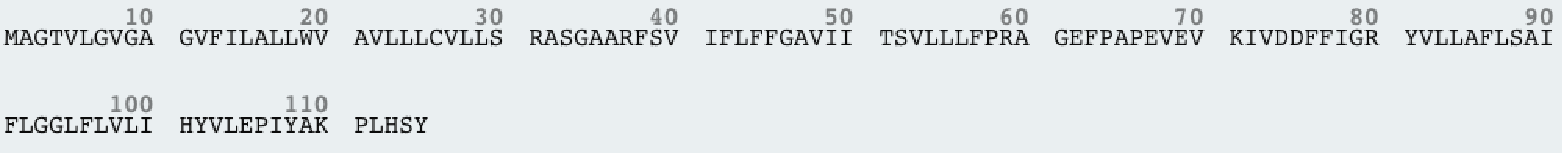
\includegraphics[width=\linewidth]{images/bg_seq.pdf}

    \caption{Transmembrane protein 218 amino acid sequence as presented by UniProt \citep{prot_A2RU14}.}

    \label{fig:sequence example} 
\end{figure}

Proteins are a linear sequence of amino acids \citep{prot_struct_lib}. An example of this sequence is the protein, Transmembrane protein 218, with a linear sequence of 115 amino acids \ref{fig:sequence example} \citep{prot_A2RU14}. There are twenty possible amino acids \citep{aa_wiki} protein sequences can be built from, and each of these amino acids have a unique side chain which have different structural properties. Different proteins have different sequences of amino acids. The amino acids in the sequence will "interact with each other to form a well-defined, folded protein" \citep{protein_folding}. The folded protein with have a three-dimensional structure, and this three-dimensional structure determines the protein's function \citep{bbc_bitesize}. This function can be supporting frameworks inside cells, catalysing biological reactions, communication between different parts of the body and proteins are used for function inside the immune system \citep{bbc_bitesize}. Therefore, it is important that the folding of proteins is done correctly as misfolded proteins will lose their structure and function, which can lead to diseases. 

\subsection{Intrinsically disordered proteins (IDPs)}
\label{chap:background sec:IDPs}

IDPs are different to structured proteins. These unstructured, disordered proteins are suggested to cause a number of diseases. Their amino acid sequences differ and contain a “low content of bulky hydrophobic amino acids and a high proportion of polar and charged amino acids” \citep{idp_wiki}. In comparison to structured proteins that fold correctly these sequences cannot fold into stable globular proteins, meaning that the protein lacks an ordered three-dimensional structure. The root cause of this lack of structure, causing disorder, is the proteins’ primary structure: the amino acid sequence. When disordered amino acids are grouped, this is labelled as an intrinsically disordered region (IDR) and is where the misfolding occurs. Therefore, making predictions about the probability that an amino acid residue is ordered or disordered within a protein sequence will help determine where this incorrect folding will occur. This means by focusing on the amino acids’ structure we can determine the outcome of the protein functioning correctly. 

A current problem is the lack of labelled data about the structure of protein sequences as determining these via experiments such as nuclear magnetic resonance (NMR) and small-angle X-ray scattering (SAXS) is very costly and time-consuming \citep{disordered_prot_genus_camelus}. To tackle this challenge, bioinformatic tools have been created for protein sequence structure labelling. These tools are often accessible via a web server, such as the DISOPRED server \citep{disopred3_paper}, which uses machine learning methods to make predictions. This project will produce a similar tool for classifying intrinsically disordered proteins after experimentation with different deep learning architectures and approaches.

\section{Deep learning overview}

\subsection{Deep Neural Networks}

Deep neural networks are made up of stacked neural network layers. As these layers are stacked, the output of one layer will be used as input to the next layer in the network. Each of these layers performs feature extraction on their input. Each layer can consist of an arbitrary number of neurons, each with their own parameter weight which is learnt during training. During training, inputs are classified by the model during a forward pass through the model. These predictions are compared to the true value using a loss function. Through the process of backpropagation \citep{Goodfellow-et-al-2016}, the outcome of the loss function is used and the parameter weights for each neuron within the network are changed in an aim to improve the models' predictions. To complete this training step, an optimisation method will update each layer of the network, changing the weights of the model as proposed by backpropagation. This training procedure is done with each item in the training set and for multiple iterations of the entire training set, to solve the optimisation problem by minimising the loss and finding optimum weights for each neuron. The machine learning framework, PyTorch \citep{pytorch}, provides the functionality to build neural network layers that extract features; use a loss function with an implemented backpropagation method, and create an optimiser to update a deep neural network model during training. PyTorch also provides efficient tensor computations and can utilise GPUs while training. This software will be useful for creating our deep neural networks due to it's efficiency and comprehensive components.

\subsection{Convolutional Neural Networks (CNNs)}

A CNN is a type of neural network that uses convolution kernels to extract features from an input. Convolution kernels can be 1D kernels of size $1\times K$ primarily used for sequence or series data, or 2D kernels of size $N\times M$ primarily used for classifying images. These kernels move across a grid shaped input, checking if a feature is present. With our protein sequences, we can use a kernel of $1\times K$ to slide along a $1\times sequence length$ grid, treating each amino acid as a different input channel and capturing unique. We can also represent protein sequences as images by creating a $20\times sequence length$ length grid, where each amino acid is a $20\times 1$ vector and this lets us use a different 2D convolution kernel over the protein sequence. These are discussed further in our design (\ref{chap:design}). 

In classification tasks convolution kernels are translation-invariant and require few parameters. These are beneficial as this means it does not matter where the location of the disordered region exists in the sequence. Less parameters means the model can be trained with smaller training sets, which is good as the labelled disorder datasets from Disprot \citep{disprot} is small in comparison to other deep learning tasks. Papers such as DISOPRED3 have stated further annotated training labels will be beneficial to prediction models \citep{disopred3_paper}; therefore, using a model that can cope with smaller datasets should be effective.

During most classification tasks, input of the same shape is passed to the CNN. However, with our protein sequence data the lengths of our sequences range from 19 \citep{prot_P0C8E0} to 34350 \citep{prot_Q8WZ42}, so we would need to unnecessarily pad many sequences with lots of redundant blank values. Therefore, we have taken an approach to use a fully convolutional network (FCN). Modern classification networks have been adapted to fully convolutional networks by Shelhamer and Long \citep{fcn_seg}, demonstrating that classification can be done using inputs of arbitrary size. Thus, for these protein sequences of varying length, an FCN will be suitable at handling these inputs. 

\subsection{Recurrent Neural Networks (RNNs)}

\section{Review of current approaches}
\label{sec:current approaches}

There are currently many approaches to protein disorder prediction, with over 100 different predictors proposed \citep{Zhao:22}. Disorder classifiers implement different methods with the main approaches regarded as: composition-based methods (PONDR VLXT \citep{Romero:01}); hydropath-based methods (DISOPRED \citep{Ward:04}); structural methods (IUPred \citep{Dosztanyi:18}); physiochemical methods (FoldIndex \citep{Prilusky:05}); machine learning methods (DISOPRED3 \citep{disopred3_paper}) and the use of meta-predictors (Metapredict \citep{Emenecker:21}). The Critical Assessment of Structure Prediction (CASP) \citep{casp} motivated solutions for identifying disordered regions in target proteins between 2010-12 using CASP9 and CASP10. Results from the CASP10 assessment \citep{CASP10} show that the top disordered region classifiers belong to machine learning and meta-predictor methods \citep{Zhao:22}. CASP has discontinued the evaluation of IDR prediction, however the Critical Assessment of Intrinsic Protein Disorder community \citep{Necci:21}, continued to release withheld testing datasets to assess new prediction tools. These assessments found that deep learning predictors had the best performance at identifying disordered regions accurately \citep{Zhao:22}. This motivates a reason for approaching this task using a deep learning method.

As well as performing well for intrinsic disorder prediction deep learning methods also dominate in other protein structure prediction tasks such as AlphaFold \citep{Jumper:21}. Improved technology has assisted these neural networks to feasibly increase their depth as well as the increase of digitalised labelled data. Studies have analysed different deep learning architectures for protein disorder prediction and state: “that the architectures of current deep learners are considerably diverse,” and there is no decided optimal architecture yet \citep{Zhao:22}. This motivates us to experiment and compare different deep learning architectures. Furthermore, the top performing models in CAID “utilize deep convolutional and/or recurrent neural networks,” \citep{Hu:21} demonstrating these architectures are important for classifiers tackling this prediction task.

\subsection{Convolutional neural networks}

A model using a convolutional neural network architecture will process the amino acid sequence in a sliding window fashion using a convolution kernel. Older competitive machine learning based methods such as DISOPRED, FoldIndex and IUPred use a sliding window within their algorithm, which justifies the feasibility of a convolution kernel. There are not many prominent models which solely use convolutional layers for protein disorder classification. However, two studies propose using a CNN for similar tasks: predicting DNA-protein binding \citep{Zeng:16}, and protein secondary structure prediction \citep{Ema:22}. The first study concludes that experimentation of different CNN architecture design demonstrated improvements to a state-of-the-art solution and this work “will be important for sequence-based tasks in genomics,” \citep{Zeng:16}. This suggests experimentation using a CNN will be useful for classification of disordered regions as we will be using a sequence-based approach with our protein sequences. The second study successfully implements a (2D) CNN with a hybrid machine learning layer and using protein sequence data for protein secondary structure prediction, which is a similar task to our protein disorder prediction problem. Although CNNs are very good at capturing local relationships, they are more limited in identifying medium and long-range sequence information. Wang et al proposes DeepCNF-D \citep{Wang:15}, which uses a deep convolutional neural fields architecture (comprising of a deep convolutional neural network and conditional random field) to reach state-of-the-art performance on the CASP benchmark datasets. The result of using a CNF architecture demonstrates the benefit of capturing complex dependencies from the amino acid sequences.

\subsection{Recurrent neural networks}

Findings that improved performance can result from capturing long-range and complex sequence dependencies that are encoded in intrinsically disordered proteins is useful. Recurrent neural networks can use their ability to maintain a hidden state to capture long-term dependencies, which is shown by the Long Short-Term Memory (LSTM) deep recurrent neural network SPOT-DISORDER \citep{Hanson:16}. This study achieved the best performance or matched best performing protein disorder prediction methods for all independent test sets and demonstrated “the capability of the LSTM technique to pick up long-range, non-local interactions” \citep{Hanson:16}. This approach also used a bidirectional recurrent neural network architecture, which is known to capture long-term dependencies and perform better than a traditional LSTM \citep{Graves:05}. Therefore, these bidirectional LSTM architectures are more likely to enhance protein disorder classification methods and should be considered with our approach.

\subsection{Ensemble approach}

As no definitive optimal architecture has been found, taking the consensus from multiple predictions using different models with different architectures can improve prediction accuracy. An improvement to the previous LSTM version of SPOT-DISORDER takes this ensemble approach, supporting that “the use of an ensemble predictor minimizes the effect of generalization errors between models” \citep{spot_disorder_2}. This SPOT-DISORDER2 ensemble uses CNN and RNN (LSTM) models, which improves prediction performance by removing “spurious false predictions” \citep{spot_disorder_2}. This paper finds benefits of using multiple models and highlights the benefit of experimenting with different architectures. These ensemble methods have also been motivated by meta-predictors which use other disorder predictors to reach a consensus prediction \citep{Emenecker:21}. These meta-approaches succeed at reaching top results and demonstrate the need for exploration of different model architectures.

\subsection{Accessibility of disorder classifiers}

Having multiple prediction models also allows researchers to create their own consensus of disorder prediction using different models. It is important that these prediction tools are easily accessible. Most trained classifiers are accessible to download and use with protein sequence data, which is beneficial for bioinformaticians. Furthermore, many studies produce an online web server to benefit less technical researchers, where they can make predictions on protein sequences using the trained classifiers via their browser. With this easy access, research can benefit from accurate predictions about protein sequences. These web servers display highlighted disordered regions within the protein sequence or graphs demonstrating the probability that a region is intrinsically disordered. This makes it clear from visual inspection where the protein is likely to misfold.

\subsection{Summary}

The findings of these current approaches demonstrate that intrinsic disorder prediction in proteins is successful with deep learning classifiers and that the exploration of different accurate models will allow for future ensemble and meta predictions to be taken. The use of protein disorder prediction by researchers also makes it clear why an easily accessible web server is important in allowing interaction with the prediction tool.


%==================================================================================================================================
\chapter{Analysis/Requirements}

\section{General deep learning problem}

In our discussion of intrinsically disordered proteins (\ref{chap:background sec:IDPs}), we demonstrate that the sequences of these proteins are different compared to ordered protein sequences. If we evaluate which amino acids appear within specific regions and where they appear, we can draw conclusions about where these disordered regions are. Therefore, we will use a supervised learning approach with our deep neural network, like current approaches, by using these amino acid sequences alongside their labelled disordered regions.  

\section{Our dataset}

As the identification of these disordered regions requires complex experimentation (\ref{chap:background}), we must use a curated database of disordered proteins. The Disprot database \citep{disprot} has been used for a variety of machine learning tasks such as the training and testing of DISOPRED3 \citep{disopred3_paper}, PONDR \citep{Xue:10}, MFDp2 \citep{Mizianty:13} and SPOT-DISORDER \citep{Hanson:16}, which all involved classifying disordered proteins. This database is regarded as the “major repository of manually curated data for intrinsically disordered proteins” \citep{Quaglia:22} and is widely used by researchers studying disordered proteins. Disprot stores information about the positions of IDRs in sequences and uses a UniProtKB accession number to identify the protein. This identifier will allow us to retrieve the full protein sequence from the UniProt database \citep{uniprot:22}, another manually curated database for proteins, to help us train our network. 

\section{Labelled data}

\begin{figure}
    \centering
    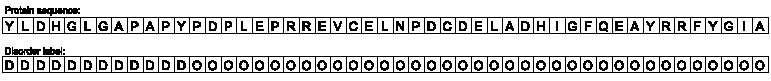
\includegraphics{images/groundtruth.pdf}    

    \caption{The Osteocalcin protein \citep{prot_Q8HYY9} and it's disorder label. This ground truth label, represents disordered amino acids with a D and ordered amino acids are represented with O. Here we see the disordered region is at the start of this small protein sequence}

    \label{fig:groundtruth} 
\end{figure}

Compared to other problems solved by deep neural networks, such as protein structure prediction \citep{Jumper:21}, classifying images \citep{Xie:17} and language modelling \citep{Devlin:18}, the size of our manually labelled dataset is much smaller. Disprot only contains around 2500 protein sequences. However, we are not classifying an entire sequence as either ordered or disordered, we are classifying a single amino acid within the sequence as ordered or disordered as seen in Figure \ref{fig:groundtruth}. This is because we know the region of the protein can be disordered due to the characteristics of the grouped amino acids. This gives us sufficient labelled data. Using these labelled sequences as our ground truth, we can utilise our deep neural networks to recognise patterns and relationships about the amino acid sequence that causes intrinsic disorder in proteins through our supervised learning approach.

\section{Approaches}

Machine learning algorithms cannot operate on our protein sequences directly. Therefore, to ensure our model is equipped to handle the various amino acids, we will consider them as distinct categories of data and employ feature encoding techniques to generate a suitable numerical input \citep{Kumar:20}.

\subsection{One-hot}

Our first feature encoding approach is one-hot encoding \citep{One-hot:wiki} \citep{Fawcett:21}. We can treat each amino acid as a vector by using the one-hot encoding technique. Our vectors will have a size of 20 because of the twenty possible amino acids, therefore as these feature vectors are not excessively large, this one-hot approach is suitable. This has let us transform a raw amino acid sequence into a feature matrix, of shape $20 \times sequence length$, which now represents the sequence.

\subsection{Position-Specific Scoring Matrix (PSSM)}

Our other feature encoding approach is to generate a position-specific scoring matrix (PSSM) \citep{PSSM:wiki}. This technique is used in many protein structure problems, such as predicting protein secondary structure \citep{McGuffin:00}, identifying sequence-contact relationships \citep{Wang:17} and used within current approaches previously discussed in our review of the literature. A PSSM is a “matrix that involves information about the probability of amino acids or nucleotides occurrence in each position, which is derived from a multiple sequence alignment” \citep{Mohammadi:22}. These PSSMs provide an informative representation about the amino acids at positions within the protein sequences which will be helpful for our network to identify patterns and relationships within protein sequences. Furthermore, as PSSMs are also of shape $20 \times sequence length$, the neural network models will be able to take both one-hot encoded sequence matrices and PSSMs as input without any changes, allowing us to compare these different feature encoding methods.

\section{Architectures}

\section{Evaluation metrics}
With our trained deep neural network, we will evaluate its predictions using similar approaches to the literature. As this is a binary classification task classifying amino acids as either ordered or disordered we can define our outcomes as: 

\begin{itemize}    
    \item True positive (TP): When the model correctly predicts that a disordered residue is disordered.
    \item True negative (TN): When the model correctly predicts that an ordered residue is ordered.
    \item False positive (FP): When the model incorrectly predicts that an ordered residue is disordered.
    \item False negative (FN): When the model incorrectly predicts that a disordered residue is ordered. \citep{google_TP}
\end{itemize}

By computing these outcomes, we can evaluate the accuracy, precision, recall (sensitivity) and specificity of our model. These metrics are widely used in various machine learning tasks as standard performance measures \citep{BC:wiki}. We can also calculate the F1-score which is the harmonic mean of the precision and recall and is another useful measure of how accurate our model is. Furthermore, as our dataset has a bias of ordered labels, we will consider the Matthews correlation coefficient (MCC), which is a more reliable measure when dealing with an imbalanced or disproportionate dataset \citep{Chicco:20}.

With these evaluation metrics we will be able to compare our approaches and architectures against each other. We can also compare our models to known current approaches using the CASP datasets which have been used for benchmarking these protein disorder prediction models \citep{casp}.

\section{Django server}

In addition to evaluating deep learning models, it is necessary to create a Django-based server that enables users to submit a protein sequence and obtain a comprehensible representation of the disordered regions of the protein. From the literature, papers proposing protein disorder prediction tools also often set up an online server so their tool can be used such as UCL's PSIPRED workbench \citep{DISOPRED:server} and the recently published Metapredict server \citep{Metapredict:server}. These protein prediction servers are important as they allow researchers to easily access these tools, allowing them to understand the structure and function of proteins which is useful for protein engineering \citep{prot_engineering:wiki}. 

A brief analysis of the server’s requirements follows following the MoSCoW prioritisation method \citep{moscow}: 
\subsection{Functional requirements}

\begin{itemize}    
    \item Must have: The server will have a web interface, so it is easily accessible for use by researchers.
    \item Must have: Users can submit a single protein sequence via a form.
    \item Must have: The server can make a prediction on a protein sequence using a deep neural network. This model will be chosen from our evaluation.
    \item Should have: The web interface will have a clear visualisation displaying the sequence to the user with clearly identified IDRs.
    \item Could have: The web interface will have a graphical representation of the identified IDRs.
    \item Will not have this time: The visualisation of the disordered sequence cannot be saved.
    \item Will not have this time: The server will not allow multiple sequences to be entered in a single form submission.
\end{itemize}

\subsection{Non-functional requirements of our server}

\begin{itemize}    
    \item Must have: The web interface will be intuitive and easy to use. Both when entering information in via the form and interpreting the outputted sequence with highlighted disordered regions.
    \item Should have: The web application should be containerised to follow best practices and be easily portable.
    \item Could have: The Django server could interact with an external database for efficient lookup of previously entered sequences and their representations.
    \item Will not have this time: The web page will not be hosted and accessible via a searchable domain by the conclusion of the project.
\end{itemize}


\newpage
What is the problem that you want to solve, and how did you arrive at it?
\section{Guidance}
Make it clear how you derived the constrained form of your problem via a clear and logical process. 

%==================================================================================================================================
\chapter{Design}
\label{chap:design}
How is this problem to be approached, without reference to specific implementation details? 
\section{Guidance}
Design should cover the abstract design in such a way that someone else might be able to do what you did, but with a different language or library or tool.

%==================================================================================================================================
\chapter{Implementation}
What did you do to implement this idea, and what technical achievements did you make?
\section{Guidance}
You can't talk about everything. Cover the high level first, then cover important, relevant or impressive details.



\section{General points}

These points apply to the whole dissertation, not just this chapter.



\subsection{Figures}
\emph{Always} refer to figures included, like Figure \ref{fig:relu}, in the body of the text. Include full, explanatory captions and make sure the figures look good on the page.
You may include multiple figures in one float, as in Figure \ref{fig:synthetic}, using \texttt{subcaption}, which is enabled in the template.



% Figures are important. Use them well.
\begin{figure}
    \centering
    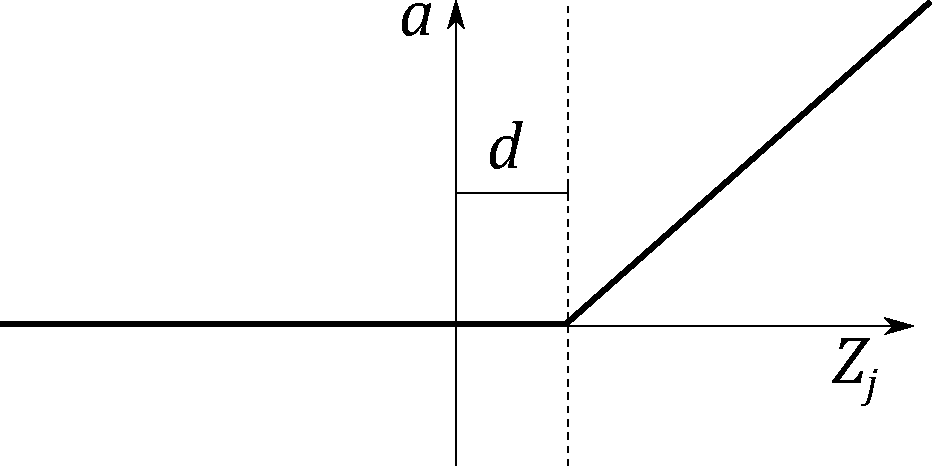
\includegraphics[width=0.5\linewidth]{images/relu.pdf}    

    \caption{In figure captions, explain what the reader is looking at: ``A schematic of the rectifying linear unit, where $a$ is the output amplitude,
    $d$ is a configurable dead-zone, and $Z_j$ is the input signal'', as well as why the reader is looking at this: 
    ``It is notable that there is no activation \emph{at all} below 0, which explains our initial results.'' 
    \textbf{Use vector image formats (.pdf) where possible}. Size figures appropriately, and do not make them over-large or too small to read.
    }

    % use the notation fig:name to cross reference a figure
    \label{fig:relu} 
\end{figure}


\begin{figure}
    \centering
    \begin{subfigure}[b]{0.45\textwidth}
        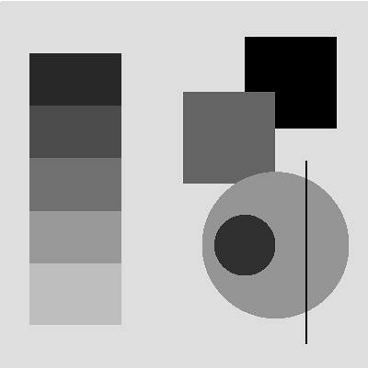
\includegraphics[width=\textwidth]{images/synthetic.png}
        \caption{Synthetic image, black on white.}
        \label{fig:syn1}
    \end{subfigure}
    ~ %add desired spacing between images, e. g. ~, \quad, \qquad, \hfill etc. 
      %(or a blank line to force the subfigure onto a new line)
    \begin{subfigure}[b]{0.45\textwidth}
        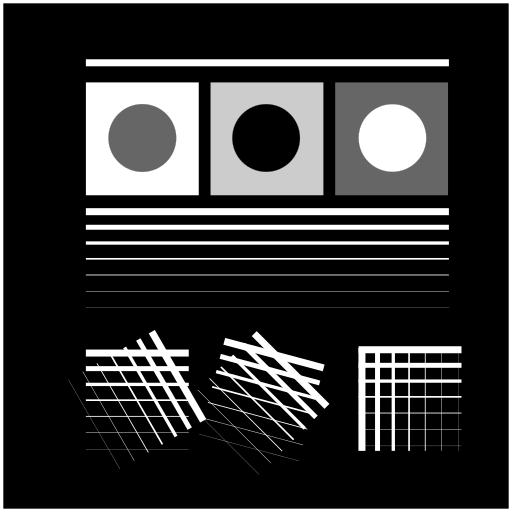
\includegraphics[width=\textwidth]{images/synthetic_2.png}
        \caption{Synthetic image, white on black.}
        \label{fig:syn2}
    \end{subfigure}
    ~ %add desired spacing between images, e. g. ~, \quad, \qquad, \hfill etc. 
    %(or a blank line to force the subfigure onto a new line)    
    \caption{Synthetic test images for edge detection algorithms. \subref{fig:syn1} shows various gray levels that require an adaptive algorithm. \subref{fig:syn2}
    shows more challenging edge detection tests that have crossing lines. Fusing these into full segments typically requires algorithms like the Hough transform.
    This is an example of using subfigures, with \texttt{subref}s in the caption.
    }\label{fig:synthetic}
\end{figure}

\clearpage

\subsection{Equations}

Equations should be typeset correctly and precisely. Make sure you get parenthesis sizing correct, and punctuate equations correctly 
(the comma is important and goes \textit{inside} the equation block). Explain any symbols used clearly if not defined earlier. 

For example, we might define:
\begin{equation}
    \hat{f}(\xi) = \frac{1}{2}\left[ \int_{-\infty}^{\infty} f(x) e^{2\pi i x \xi} \right],
\end{equation}    
where $\hat{f}(\xi)$ is the Fourier transform of the time domain signal $f(x)$.

\subsection{Algorithms}
Algorithms can be set using \texttt{algorithm2e}, as in Algorithm \ref{alg:metropolis}.

% NOTE: line ends are denoted by \; in algorithm2e
\begin{algorithm}
    \DontPrintSemicolon
    \KwData{$f_X(x)$, a probability density function returing the density at $x$.\; $\sigma$ a standard deviation specifying the spread of the proposal distribution.\;
    $x_0$, an initial starting condition.}
    \KwResult{$s=[x_1, x_2, \dots, x_n]$, $n$ samples approximately drawn from a distribution with PDF $f_X(x)$.}
    \Begin{
        $s \longleftarrow []$\;
        $p \longleftarrow f_X(x)$\;
        $i \longleftarrow 0$\;
        \While{$i < n$}
        {
            $x^\prime \longleftarrow \mathcal{N}(x, \sigma^2)$\;
            $p^\prime \longleftarrow f_X(x^\prime)$\;
            $a \longleftarrow \frac{p^\prime}{p}$\;
            $r \longleftarrow U(0,1)$\;
            \If{$r<a$}
            {
                $x \longleftarrow x^\prime$\;
                $p \longleftarrow f_X(x)$\;
                $i \longleftarrow i+1$\;
                append $x$ to $s$\;
            }
        }
    }
    
\caption{The Metropolis-Hastings MCMC algorithm for drawing samples from arbitrary probability distributions, 
specialised for normal proposal distributions $q(x^\prime|x) = \mathcal{N}(x, \sigma^2)$. The symmetry of the normal distribution means the acceptance rule takes the simplified form.}\label{alg:metropolis}
\end{algorithm}

\subsection{Tables}

If you need to include tables, like Table \ref{tab:operators}, use a tool like https://www.tablesgenerator.com/ to generate the table as it is
extremely tedious otherwise. 

\begin{table}[]
    \caption{The standard table of operators in Python, along with their functional equivalents from the \texttt{operator} package. Note that table
    captions go above the table, not below. Do not add additional rules/lines to tables. }\label{tab:operators}
    %\tt 
    \rowcolors{2}{}{gray!3}
    \begin{tabular}{@{}lll@{}}
    %\toprule
    \textbf{Operation}    & \textbf{Syntax}                & \textbf{Function}                            \\ %\midrule % optional rule for header
    Addition              & \texttt{a + b}                          & \texttt{add(a, b)}                                    \\
    Concatenation         & \texttt{seq1 + seq2}                    & \texttt{concat(seq1, seq2)}                           \\
    Containment Test      & \texttt{obj in seq}                     & \texttt{contains(seq, obj)}                           \\
    Division              & \texttt{a / b}                          & \texttt{div(a, b) }  \\
    Division              & \texttt{a / b}                          & \texttt{truediv(a, b) } \\
    Division              & \texttt{a // b}                         & \texttt{floordiv(a, b)}                               \\
    Bitwise And           & \texttt{a \& b}                         & \texttt{and\_(a, b)}                                  \\
    Bitwise Exclusive Or  & \texttt{a \textasciicircum b}           & \texttt{xor(a, b)}                                    \\
    Bitwise Inversion     & \texttt{$\sim$a}                        & \texttt{invert(a)}                                    \\
    Bitwise Or            & \texttt{a | b}                          & \texttt{or\_(a, b)}                                   \\
    Exponentiation        & \texttt{a ** b}                         & \texttt{pow(a, b)}                                    \\
    Identity              & \texttt{a is b}                         & \texttt{is\_(a, b)}                                   \\
    Identity              & \texttt{a is not b}                     & \texttt{is\_not(a, b)}                                \\
    Indexed Assignment    & \texttt{obj{[}k{]} = v}                 & \texttt{setitem(obj, k, v)}                           \\
    Indexed Deletion      & \texttt{del obj{[}k{]}}                 & \texttt{delitem(obj, k)}                              \\
    Indexing              & \texttt{obj{[}k{]}}                     & \texttt{getitem(obj, k)}                              \\
    Left Shift            & \texttt{a \textless{}\textless b}       & \texttt{lshift(a, b)}                                 \\
    Modulo                & \texttt{a \% b}                         & \texttt{mod(a, b)}                                    \\
    Multiplication        & \texttt{a * b}                          & \texttt{mul(a, b)}                                    \\
    Negation (Arithmetic) & \texttt{- a}                            & \texttt{neg(a)}                                       \\
    Negation (Logical)    & \texttt{not a}                          & \texttt{not\_(a)}                                     \\
    Positive              & \texttt{+ a}                            & \texttt{pos(a)}                                       \\
    Right Shift           & \texttt{a \textgreater{}\textgreater b} & \texttt{rshift(a, b)}                                 \\
    Sequence Repetition   & \texttt{seq * i}                        & \texttt{repeat(seq, i)}                               \\
    Slice Assignment      & \texttt{seq{[}i:j{]} = values}          & \texttt{setitem(seq, slice(i, j), values)}            \\
    Slice Deletion        & \texttt{del seq{[}i:j{]}}               & \texttt{delitem(seq, slice(i, j))}                    \\
    Slicing               & \texttt{seq{[}i:j{]}}                   & \texttt{getitem(seq, slice(i, j))}                    \\
    String Formatting     & \texttt{s \% obj}                       & \texttt{mod(s, obj)}                                  \\
    Subtraction           & \texttt{a - b}                          & \texttt{sub(a, b)}                                    \\
    Truth Test            & \texttt{obj}                            & \texttt{truth(obj)}                                   \\
    Ordering              & \texttt{a \textless b}                  & \texttt{lt(a, b)}                                     \\
    Ordering              & \texttt{a \textless{}= b}               & \texttt{le(a, b)}                                     \\
    % \bottomrule
    \end{tabular}
    \end{table}
\subsection{Code}

Avoid putting large blocks of code in the report (more than a page in one block, for example). Use syntax highlighting if possible, as in Listing \ref{lst:callahan}.

\begin{lstlisting}[language=python, float, caption={The algorithm for packing the $3\times 3$ outer-totalistic binary CA successor rule into a 
    $16\times 16\times 16\times 16$ 4 bit lookup table, running an equivalent, notionally 16-state $2\times 2$ CA.}, label=lst:callahan]
    def create_callahan_table(rule="b3s23"):
        """Generate the lookup table for the cells."""        
        s_table = np.zeros((16, 16, 16, 16), dtype=np.uint8)
        birth, survive = parse_rule(rule)

        # generate all 16 bit strings
        for iv in range(65536):
            bv = [(iv >> z) & 1 for z in range(16)]
            a, b, c, d, e, f, g, h, i, j, k, l, m, n, o, p = bv

            # compute next state of the inner 2x2
            nw = apply_rule(f, a, b, c, e, g, i, j, k)
            ne = apply_rule(g, b, c, d, f, h, j, k, l)
            sw = apply_rule(j, e, f, g, i, k, m, n, o)
            se = apply_rule(k, f, g, h, j, l, n, o, p)

            # compute the index of this 4x4
            nw_code = a | (b << 1) | (e << 2) | (f << 3)
            ne_code = c | (d << 1) | (g << 2) | (h << 3)
            sw_code = i | (j << 1) | (m << 2) | (n << 3)
            se_code = k | (l << 1) | (o << 2) | (p << 3)

            # compute the state for the 2x2
            next_code = nw | (ne << 1) | (sw << 2) | (se << 3)

            # get the 4x4 index, and write into the table
            s_table[nw_code, ne_code, sw_code, se_code] = next_code

        return s_table

\end{lstlisting}

%==================================================================================================================================
\chapter{Evaluation} 
How good is your solution? How well did you solve the general problem, and what evidence do you have to support that?

\section{Guidance}
\begin{itemize}
    \item
        Ask specific questions that address the general problem.
    \item
        Answer them with precise evidence (graphs, numbers, statistical
        analysis, qualitative analysis).
    \item
        Be fair and be scientific.
    \item
        The key thing is to show that you know how to evaluate your work, not
        that your work is the most amazing product ever.
\end{itemize}

\section{Evidence}
Make sure you present your evidence well. Use appropriate visualisations, reporting techniques and statistical analysis, as appropriate.

If you visualise, follow the basic rules, as illustrated in Figure \ref{fig:boxplot}:
\begin{itemize}
\item Label everything correctly (axis, title, units).
\item Caption thoroughly.
\item Reference in text.
\item \textbf{Include appropriate display of uncertainty (e.g. error bars, Box plot)}
\item Minimize clutter.
\end{itemize}

See the file \texttt{guide\_to\_visualising.pdf} for further information and guidance.

\begin{figure}
    \centering
    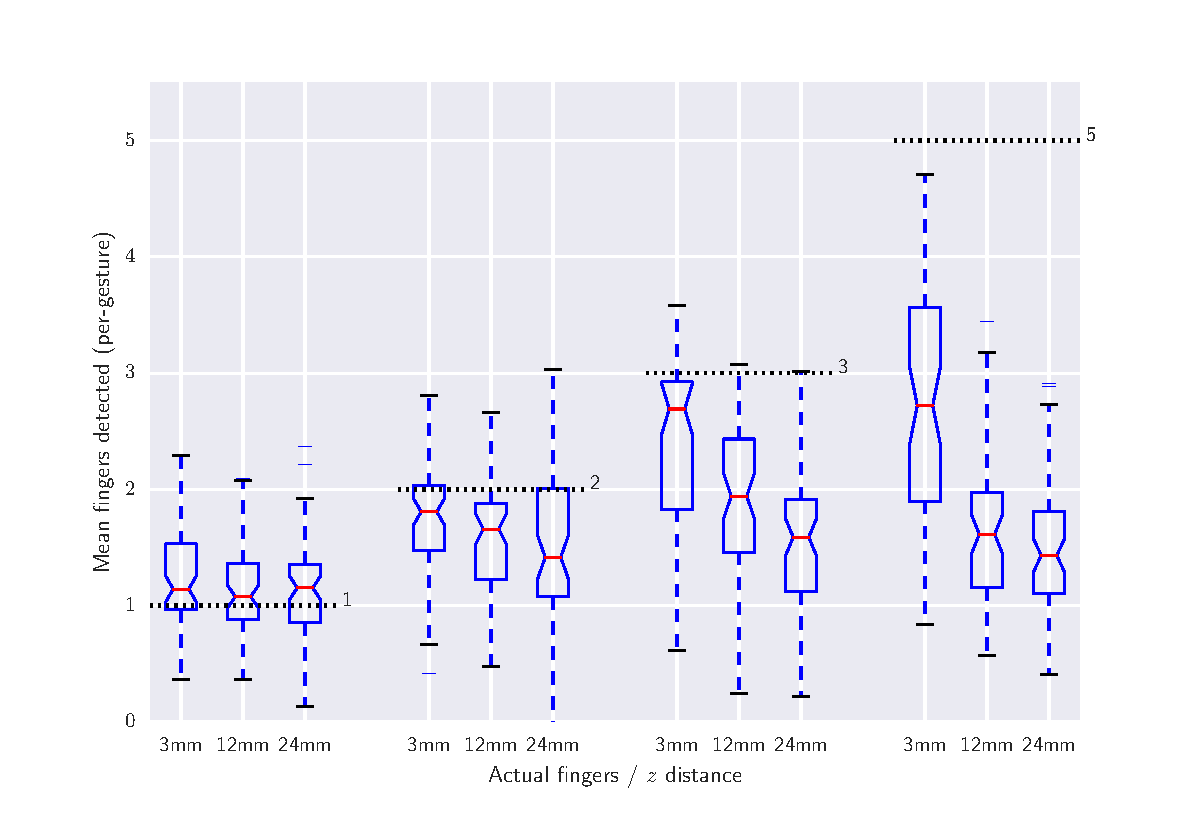
\includegraphics[width=1.0\linewidth]{images/boxplot_finger_distance.pdf}    

    \caption{Average number of fingers detected by the touch sensor at different heights above the surface, averaged over all gestures. Dashed lines indicate
    the true number of fingers present. The Box plots include bootstrapped uncertainty notches for the median. It is clear that the device is biased toward 
    undercounting fingers, particularly at higher $z$ distances.
    }

    % use the notation fig:name to cross reference a figure
    \label{fig:boxplot} 
\end{figure}


%==================================================================================================================================
\chapter{Conclusion}    
Summarise the whole project for a lazy reader who didn't read the rest (e.g. a prize-awarding committee).
\section{Guidance}
\begin{itemize}
    \item
        Summarise briefly and fairly.
    \item
        You should be addressing the general problem you introduced in the
        Introduction.        
    \item
        Include summary of concrete results (``the new compiler ran 2x
        faster'')
    \item
        Indicate what future work could be done, but remember: \textbf{you
        won't get credit for things you haven't done}.
\end{itemize}

%==================================================================================================================================
%
% 
%==================================================================================================================================
%  APPENDICES  

\begin{appendices}

\chapter{Appendices}

Typical inclusions in the appendices are:

\begin{itemize}
\item
  Copies of ethics approvals (required if obtained)
\item
  Copies of questionnaires etc. used to gather data from subjects.
\item
  Extensive tables or figures that are too bulky to fit in the main body of
  the report, particularly ones that are repetitive and summarised in the body.

\item Outline of the source code (e.g. directory structure), or other architecture documentation like class diagrams.

\item User manuals, and any guides to starting/running the software.

\end{itemize}

\textbf{Don't include your source code in the appendices}. It will be
submitted separately.

\end{appendices}

%==================================================================================================================================
%   BIBLIOGRAPHY   

% The bibliography style is abbrvnat
% The bibliography always appears last, after the appendices.

\bibliographystyle{abbrvnat}

\bibliography{l4proj}

\end{document}
